\apendice{Especificación de diseño}
\section{Introducción}

En este apéndice se mostrarán la estructura de los datos, a nivel de base de datos y a nivel de tabla/colección (tanto en MongoDB como en SQLite). Además se detallará la arquitectura del proyecto.

\section{Diseño de datos}

\subsection{Datos en MongoDB}

La base de datos MongoDB recibe el nombre de ``pisos'' y de divide en las siguientes colecciones:

\begin{itemize}
	\item \texttt{amount\_parsed}

    Esta colección sirve para monitorizar de cuantos inmuebles nuevos se introducen en la base de datos en cada ejecución del \textit{scraper}. Se crea un nuevo documento en cada ejecución con la fecha de finalización y el número de inmuebles almacenados en dicha ejecución.

	\item \texttt{last\_updated\_dates}

    Colección operacional donde se almacenan la fecha del inmueble más reciente de cada colección. Se usa para que cuando el \textit{scraper} llegue a inmuebles actualizados menos recientemente, para de operar. Por ejemplo, si para la colección de Jaén, la última fecha de actualización es el 20 de Enero de 2024, si el \textit{scraper} encuentra un inmueble del 19 de Enero de 2024, se detecta que no es necesario seguir extrayendo datos para esa provincia, ya que ya estarán insertados en la base de datos. Esto funciona porque se acceden a los inmuebles en orden de última actualización decreciente en \url{www.pisos.com}.


	\item \texttt{\{nombre\_de\_provincia\}}
 
    En estas es donde se alojan los documentos de inmuebles para cada provincia. Las colecciones que existen son las siguientes:

      a\_coruna, alava\_araba, albacete, alicante, almeria, andorra, asturias, avila, badajoz,
  barcelona, burgos, caceres, cadiz, cantabria, castellon\_castello, ceuta, ciudad\_real,
  cordoba, cuenca, girona, granada, guadalajara, guipuzcoa\_gipuzkoa, 
  huelva, huesca, islas\_baleares\_illes\_balears, jaen, la\_rioja, las\_palmas, leon, lleida, lugo, madrid,
  malaga, melilla, murcia, navarra\_nafarroa, ourense, palencia, pontevedra, salamanca,
  santa\_cruz\_de\_tenerife, segovia, sevilla, soria, tarragona, teruel, toledo, valencia,
  valladolid, vizcaya\_bizkaia, zamora, zaragoza

\end{itemize}



Se debe señalar que los campos de datos de \textit{scraping} cambian según el documento (Ver Figura \ref{fig:documento_inmueble} para ejemplo), según si hay más detalles listados en el anuncio o menos, aunque todos siguen un patrón similar. Además merece la pena señalar que todos los campos provenientes de \textit{scraping} se almacenan como cadenas de texto, para posteriormente darle tipado en la ETL con carga en la base de datos SQLite. Los campos operacionales esenciales presentes en todos los documentos son los siguientes:

\begin{itemize}
	\item{\texttt{id}: Id extraida del portal pisos.com que sirve como identificador único de principio a fin del flujo de datos}
    \item{\texttt{updated\_date}: Fecha de actualización del anuncio extraida del portal pisos.com}
    \item{\texttt{createdAt}: Momento en el que se almacenó por primera vez el inmueble en la base de datos}
    \item{\texttt{updatedAt}: Momento en el que se actualizó por última vez el documento en la base de datos}
    \item{\texttt{version}: Indica cuantas veces se ha actualizado el documento, comienza en 0 con incrementos +1}
    \item{\texttt{active}: Booleano que indica si el anuncio sigue activo o no}
\end{itemize}


\begin{figure}[ht]
    \centering
	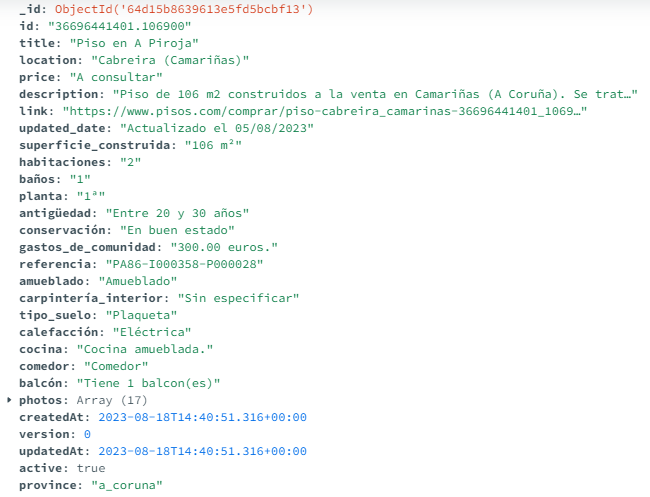
\includegraphics[width=1\textwidth]{img/documento_mongodb.PNG}
	\caption[Ejemplo de documento almacenado en base de datos MongoDB]{Ejemplo de documento almacenado en base de datos MongoDB que representa los datos de un inmueble en la colección ``a\_coruna''}
	\label{fig:documento_inmueble}
\end{figure}


\subsection{Datos en SQLite}

Tras un proceso de transformación los datos de la base de datos MongoDB se cargan en esta base de datos que consta principalmente de tres tablas:

\subsubsection{Tabla \texttt{last\_updated\_dates}}

Tabla operacional simple que almacena una columna con el nombre de la colección (de MongoDB) y otra con el tiempo de actualización (\texttt{updated\_at}) más reciente de dicha colección. Sirve para continuar el proceso de ETL en la siguiente iteración.

\subsubsection{Tabla \texttt{pisos}}{\label{subsec:tabla_pisos}}

Consta de los datos de inmuebles ya limpiados y transformados. Sirve tanto para el entrenamiento y predicción de los modelos de Aprendizaje Automático, como punto de partida de los datos agregados y para listar los inmuebles en el sitio web. 

Algunas columnas que merece la pena mencionar por su importancia operacional son: 

\begin{itemize}
\item \texttt{id} : Identificador único proveniente de pisos.com
\item \texttt{province} : La provincia del inmueble y por tanto su colección de MongoDB.
\item \texttt{capital} : Tiene valor 1 si pertenece a la capital de provincia, 0 si no.
\item \texttt{type} : Tipo de inmueble, por ejemplo Piso, Casa, Apartamento...
\item \texttt{price\_euro} : El precio de venta anunciado, incluye descuentos.
\item \texttt{link} : Enlace al inmueble en pisos.com.
\item \texttt{updated\_date} : Fecha actualización del anuncio reflejada en pisos.com.
\item \texttt{active} : Tiene valor 1 si el inmueble está considerado activo, 0 si no. Resultado del flujo de Scrapy que comprueba si el anuncio sigue activo.
\item \texttt{createdat} : Fecha de primera carga en MongoDB.
\item \texttt{updatedat} : Fecha de última actualización en MongoDB.
\item \texttt{version} : Indicador de cuantas veces se ha actualizado el inmueble en MongoDB.
\item \texttt{prediction} : Valor en € asignado por los modelos de Aprendizaje Automático.
\item \texttt{predictionupdatedat} : Tiempo en el que se actualizó el campo \texttt{prediction}.
\item \texttt{rating} : Valor calculado a través de \texttt{prediction} y \texttt{price\_euro}, explicado en \ref{sec:ml_section}). Sirve para ordenar los inmuebles de mayor a menor oportunidad.
\end{itemize}

En esta tabla, encontramos otros muchos campos que se pueden consultar en detalle en Tabla \ref{tab:schema_pisos}. Cabe mencionar que no todos los inmuebles presentan todos los campos, dependerá de cuales estén listados en el anuncio original, así encontramos muchos de ellos con valor \texttt{null}.

Finalmente, merece la pena mencionar que observamos algunos valores calculados que llevan el sufijo \texttt{\_summary} (marcado como \texttt{\_summ} en la tabla de referencia \ref{tab:schema_pisos}) o \texttt{\_cleaned}, estos datos son reagrupaciones de las mismas columnas sin sufijo que se pueden ver en la tabla, generalmente se trata de campos consolidados para su uso en los modelos. Se ha considerado que merece la pena mantener en la misma tabla los campos sin consolidar (más fieles al anuncio original) y consolidados.


\begin{longtable}{lll}
\caption{Esquema completo de la tabla \texttt{pisos}} \label{tab:schema_pisos} \\
\toprule
\textbf{Columna} & \textbf{Tipo} & \textbf{Desc.} \\
\midrule
\endfirsthead

\multicolumn{3}{c}%
{{\bfseries \tablename\ \thetable{} -- continuación de la página anterior}} \\
\toprule
\textbf{Columna} & \textbf{Tipo} & \textbf{Desc.} \\
\midrule
\endhead

\midrule
\multicolumn{3}{r}{{Continúa en la siguiente página}} \\
\endfoot

\bottomrule
\endlastfoot
id & TEXT & ID único \\
title & TEXT & Título \\
location & TEXT & Ubicación \\
province & TEXT & Provincia \\
capital & INTEGER & 0 No, 1 Yes \\
price\_euro & REAL & Precio € \\
description & TEXT & Descripción \\
link & TEXT & Enlace \\
updated\_date & TEXT & Fecha act. \\
sup.\_constr.\_m2 & REAL & Sup. constr. m² \\
sup.\_util\_m2 & REAL & Sup. útil m² \\
habitaciones & REAL & Habitaciones \\
banos & REAL & Baños \\
planta & TEXT & Planta \\
exterior & TEXT & Exterior \\
antiguedad & TEXT & Antigüedad \\
conservacion & TEXT & Conservación \\
referencia & TEXT & Ref. \\
terraza & TEXT & Terraza \\
photos & TEXT & Fotos \\
createdat & INTEGER & Creado \\
version & INTEGER & Versión \\
updatedat & INTEGER & Actualizado \\
active & INTEGER & Activo \\
amueblado & TEXT & Amueblado \\
armarios\_empotrados & TEXT & Armarios \\
tipo\_suelo & TEXT & Suelo \\
vidrios\_dobles & TEXT & Vidrios dobles \\
carpinteria\_exterior & TEXT & Carp. exterior \\
aire\_acondicionado & TEXT & Aire acond. \\
cocina & TEXT & Cocina \\
comedor & TEXT & Comedor \\
garaje & TEXT & Garaje \\
trastero & TEXT & Trastero \\
puerta\_blindada & TEXT & Puerta blindada \\
ascensor & TEXT & Ascensor \\
orientacion & TEXT & Orientación \\
soleado & TEXT & Soleado \\
chimenea & TEXT & Chimenea \\
piscina & TEXT & Piscina \\
gastos\_de\_comunidad & TEXT & Gastos com. \\
agua & TEXT & Agua \\
calefaccion & TEXT & Calefacción \\
old\_price\_euro & REAL & Precio antiguo € \\
sistema\_de\_seguridad & TEXT & Seguridad \\
balcon & TEXT & Balcón \\
superficie\_solar\_m2 & REAL & Sup. solar m² \\
tipo\_de\_casa & TEXT & Tipo de casa \\
urbanizado & TEXT & Urbanizado \\
calle\_alumbrada & TEXT & Calle alumbrada \\
calle\_asfaltada & TEXT & Calle asfaltada \\
portero\_automatico & TEXT & Portero autom. \\
adaptado\_movilidad\_reducida & TEXT & Adapt. movilidad \\
jardin & TEXT & Jardín \\
lavadero & TEXT & Lavadero \\
se\_aceptan\_mascotas & TEXT & Mascotas \\
telefono & TEXT & Teléfono \\
luz & TEXT & Luz \\
cocina\_equipada & TEXT & Cocina equip. \\
carpinteria\_interior & TEXT & Carp. interior \\
interior & TEXT & Interior \\
gas & TEXT & Gas \\
no\_se\_aceptan\_mascotas & TEXT & No mascotas \\
esquina & TEXT & Esquina \\
exterior\_summ & TEXT & Resumen exterior \\
vidrios\_dobles\_summ & TEXT & Resumen vidrios \\
adapt.\_mov.\_redu.\_summ & TEXT & Resumen adapt. movilidad \\
puerta\_blindada\_summ & TEXT & Resumen puerta blindada \\
ascensor\_summ & TEXT & Resumen ascensor \\
balcon\_summ & TEXT & Resumen balcón \\
portero\_automatico\_summ & TEXT & Resumen portero \\
garaje\_summ & TEXT & Resumen garaje \\
comedor\_summ & TEXT & Resumen comedor \\
terraza\_summ & TEXT & Resumen terraza \\
jardin\_summ & TEXT & Resumen jardín \\
armarios\_empotrados\_summ & TEXT & Resumen armarios \\
aire\_acondicionado\_summ & TEXT & Resumen aire acond. \\
trastero\_summ & TEXT & Resumen trastero \\
piscina\_summ & TEXT & Resumen piscina \\
chimenea\_summ & TEXT & Resumen chimenea \\
lavadero\_summ & TEXT & Resumen lavadero \\
urbanizado\_summ & TEXT & Resumen urbanizado \\
calle\_alumbrada\_summ & TEXT & Resumen calle alumbrada \\
calle\_asfaltada\_summ & TEXT & Resumen calle asfaltada \\
soleado\_summ & TEXT & Resumen soleado \\
gas\_summ & TEXT & Resumen gas \\
sistema\_de\_seguridad\_summ & TEXT & Resumen seguridad \\
interior\_summ & TEXT & Resumen interior \\
esquina\_summ & TEXT & Resumen esquina \\
amueblado\_summ & TEXT & Resumen amueblado \\
cocina\_equipada\_summ & TEXT & Resumen cocina equip. \\
mascotas\_summ & TEXT & Resumen mascotas \\
gastos\_de\_comunidad\_cleaned & REAL & Gastos com. limpios \\
carpinteria\_exterior\_cleaned & TEXT & Carp. exterior limpia \\
tipo\_suelo\_summ & TEXT & Resumen suelo \\
calefaccion\_summ & TEXT & Resumen calefacción \\
cocina\_summ & TEXT & Resumen cocina \\
orientacion\_summ & TEXT & Resumen orientación \\
agua\_summ & TEXT & Resumen agua \\
type & TEXT & Tipo \\
alcantarillado & TEXT & Alcantarillado \\
alcantarillado\_summ & TEXT & Resumen alcantarillado \\
prediction & REAL & Predicción \\
predictionupdatedat & TIMESTAMP & Fecha act. predicción \\
rating & REAL & Valoración \\
\end{longtable}
    
\subsubsection{Tabla \texttt{pisos\_dw}}{\label{subsec:pisos_dw}}

Esta tabla es el resultado del proceso de agregación de datos de la ETL, por lo tanto, se recalcula entera dos veces al día. Su objetivo principal es precalcular datos agregados para las visualizaciones, evitando la necesidad de computar estos datos en la web cada vez que el usuario haga una petición, como por ejemplo, al cambiar los filtros en la pestaña \textit{``VISUALIZA''}. Su origen único siempre es la tabla \texttt{pisos}.

Encontraremos todos los campos agrupados por:

\begin{itemize}
    \item \texttt{province\_group}: Provincia. Obtenido de \texttt{province} de tabla \texttt{pisos}.
    \item \texttt{capital\_group}: Si pertenecen a Capital de Provincia o no. Obtenido de \texttt{capital} de tabla \texttt{pisos}.
    \item \texttt{active\_group}: Si están en anuncios activos o no. Obtenido de \texttt{active} de tabla \texttt{pisos}.
    \item \texttt{updated\_month\_group}:  Mes-Año en el que se insertaron por primera vez en MongoDB (calculado desde campo \texttt{createdat} de tabla \texttt{pisos})
\end{itemize}

Además, para cada agrupación, existe un valor \texttt{'all'}, que identifica el cálculo sin tener en cuenta dicha agrupación. Por ejemplo, si todas las agrupaciones tienen valor \texttt{'all'} los cálculos agregados pertenecerán a todos los inmuebles de la base de datos, sin tener en cuenta provincia, capital, activos o tiempo de creación. 

Para algunas columnas provenientes de tabla \texttt{pisos}, denominadas como \textbf{numéricas} (Ver en Tabla \ref{tab:numerical_columns_pisosdw}), se calculan la media y la desviación estándar, descartando los \textit{outliers} para el cálculo.

El cálculo de \textit{outliers} se realiza teniendo en cuenta unos límites superiores e inferiores muy restrictivos, ya que no queremos eliminar muchos datos. Siendo $q1$ el cuartil 1, $q3$ el cuartil 3, e $iqr = q3 - q1$, los límites se definen como:

\begin{align*}
\text{Límite inferior} &= q1 - 5 \times iqr \\
\text{Límite superior} &= q3 + 5 \times iqr
\end{align*}

Para el resto de columnas provenientes de tabla \texttt{pisos}, denominadas como \textbf{categóricas} (Ver en Tabla \ref{tab:categorical_columns_pisosdw}), lo que se hace es calcular qué porcentaje de los inmuebles adquiere cada valor único posible, también siendo agrupados según los grupos mencionados previamente.

Por ejemplo para \texttt{piscina\_summary} los valores posibles son \texttt{YES} o \texttt{NO}. Se calculará que porcentaje de los inmuebles tienen cada uno de los valores, y se almacenarán dichos porcentajes en columnas distintas para cada valor único, que en este caso reciben el nombre de \texttt{piscina\_summary\_yes\_pct} y \texttt{piscina\_summary\_no\_pct}. Debemos tener en cuenta que estos porcentajes se calculan para cada combinación de agrupaciones, siendo así cada fila de la tabla una combinación distinta de agrupaciones.

\begin{table}[h]
\centering
\begin{tabular}{@{}ll@{}}
\toprule
\textbf{Columnas} & \\
\midrule
\texttt{price\_euro} & \texttt{superficie\_construida\_m2} \\
\texttt{superficie\_util\_m2} & \texttt{superficie\_solar\_m2} \\
\texttt{habitaciones} & \texttt{banos} \\
\texttt{gastos\_de\_comunidad\_cleaned} &  \\
\bottomrule
\end{tabular}
\caption[Columnas numéricas de la tabla \texttt{pisos} usadas para tabla agrupada \texttt{pisos\_dw}]{Columnas o campos numéricos de la tabla \texttt{pisos} usados para tabla agrupada \texttt{pisos\_dw}. Se muestran en dos grupos de columnas, para comprimir esta tabla.}
\label{tab:numerical_columns_pisosdw}
\end{table}

\begin{table}[h]
\centering
\begin{tabular}{@{}ll@{}}
\toprule
\textbf{Columnas} &  \\
\midrule
\texttt{exterior\_summary} & \texttt{comedor\_summary} \\
\texttt{vidrios\_dobles\_summary} & \texttt{terraza\_summary} \\
\texttt{adaptado\_...\_reducida\_summary} & \texttt{jardin\_summary} \\
\texttt{puerta\_blindada\_summary} & \texttt{armarios\_empotrados\_summary} \\
\texttt{ascensor\_summary} & \texttt{aire\_acondicionado\_summary} \\
\texttt{balcon\_summary} & \texttt{trastero\_summary} \\
\texttt{portero\_automatico\_summary} & \texttt{piscina\_summary} \\
\texttt{garaje\_summary} & \texttt{chimenea\_summary} \\
\texttt{lavadero\_summary} & \texttt{soleado\_summary} \\
\texttt{gas\_summary} & \texttt{amueblado\_summary} \\
\texttt{cocina\_equipada\_summary} & \texttt{calefaccion\_summary} \\
\texttt{conservacion} & \texttt{antiguedad} \\
\texttt{carpinteria\_exterior\_cleaned} & \texttt{tipo\_suelo\_summary} \\
\texttt{cocina\_summary} & \texttt{orientacion\_summary} \\
\bottomrule
\end{tabular}
\caption[Columnas categóricas de la tabla \texttt{pisos} usadas para tabla agrupada \texttt{pisos\_dw}]{Columnas o campos categóricos de la tabla \texttt{pisos} usados para tabla agrupada \texttt{pisos\_dw}. Se muestran en dos grupos de columnas, para comprimir esta tabla.}
\label{tab:categorical_columns_pisosdw}
\end{table}

\clearpage
\section{Diseño de Arquitectura de Software}

El diagrama de componentes se muestra en la Figura \ref{fig:arquitectura_general}. Englobando todos los componentes, encontramos un bloque en forma de elipse que representa la máquina virtual del proyecto. Este bloque a su vez contiene dos bloques rectangulares, uno que representa los servicios relacionados con los datos (\textit{Data Services}) y otro, los relacionados con la web (\textit{Web Services}). 

Dentro de estos bloques encontramos que cada contenedor de Docker se representa como un bloque con título en azul, cada volumen se representa con un bloque con título en morado. Encontramos las diferentes tareas (con sufijo \texttt{\_task}) englobando a distintos contenedores, y la frecuencia de la tarea se representa en un bloque con forma de nube.

\begin{figure} 
    \centering
    \begin{adjustbox}{center}
	    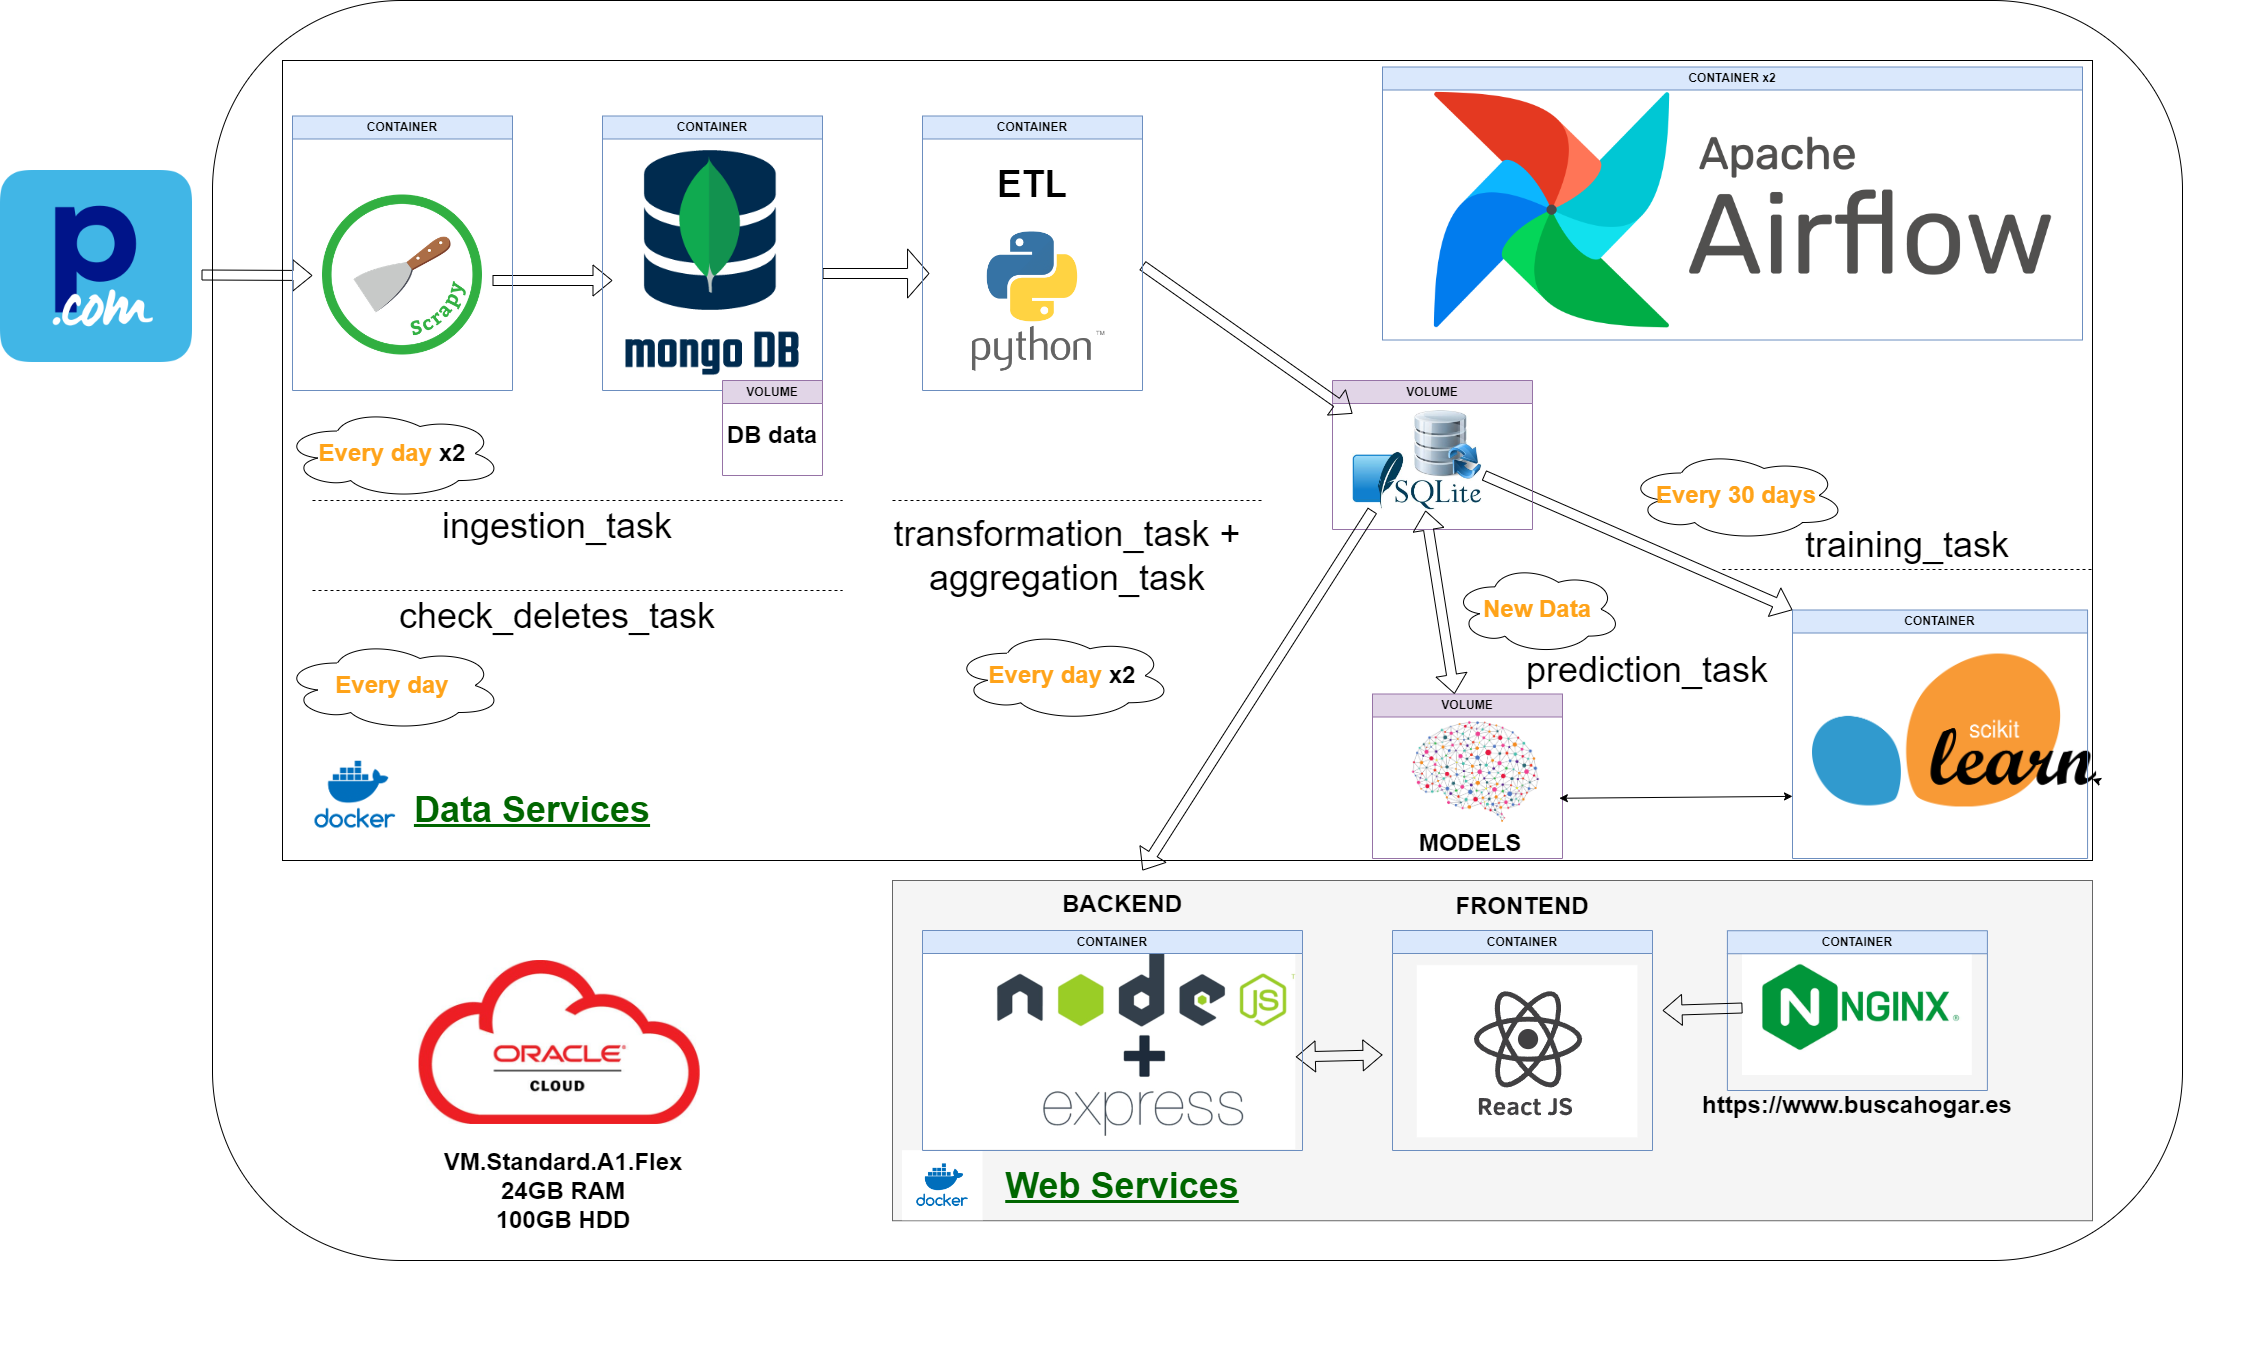
\includegraphics[width=1.1\textwidth]{img/arquitectura.png}
    \end{adjustbox}
    \caption{Arquitectura de software del proyecto}
    \label{fig:arquitectura_general}
\end{figure}
\clearpage 


